% This LaTeX document needs to be compiled with XeLaTeX.
\documentclass[10pt]{article}
\usepackage[utf8]{inputenc}
\usepackage{ucharclasses}
\usepackage{amsmath}
\usepackage{amsfonts}
\usepackage{amssymb}
\usepackage[version=4]{mhchem}
\usepackage{stmaryrd}
\usepackage{graphicx}
\usepackage[export]{adjustbox}
\graphicspath{ {./images/} }
\usepackage{bbold}
\usepackage{caption}
\usepackage[fallback]{xeCJK}
\usepackage{polyglossia}
\usepackage{fontspec}
\IfFontExistsTF{Noto Serif CJK JP}
{\setCJKmainfont{Noto Serif CJK JP}}
{\IfFontExistsTF{STSong}
  {\setCJKmainfont{STSong}}
  {\IfFontExistsTF{Droid Sans Fallback}
    {\setCJKmainfont{Droid Sans Fallback}}
    {\setCJKmainfont{SimSun}}
}}

\setmainlanguage{english}
\setotherlanguages{bahasa}
\IfFontExistsTF{CMU Serif}
{\newfontfamily\lgcfont{CMU Serif}}
{\IfFontExistsTF{DejaVu Sans}
  {\newfontfamily\lgcfont{DejaVu Sans}}
  {\newfontfamily\lgcfont{Georgia}}
}
\setDefaultTransitions{\lgcfont}{}

\def\Perp{\perp\!\!\!\perp}

\begin{document}
\captionsetup{singlelinecheck=false}
\section*{Open Systems}
a quanium state can hols less information than a deterministic state. in that case the state is (noi) pore an ne aescribe it as a frobabilistic distribution (hixture) of pure states

$$
\begin{gathered}
\frac{\text { PURE }}{|\psi\rangle} \longrightarrow \frac{\text { MIXED }}{\left(p_{\alpha},\left|\psi_{\alpha}\right\rangle\right)} \\
\text { NOT NEESSARY ORTHOKONGL }
\end{gathered}
$$

observables

$$
\begin{aligned}
&\langle\theta\rangle=\sum_{1} p_{\alpha}\left\langle\psi_{\alpha}\right| \theta\left|\psi_{\alpha}\right\rangle=\sum_{1} p_{\alpha} \operatorname{Tr}\left[\theta\left|\widetilde{\psi}_{\alpha}\right\rangle\left\langle\psi_{\alpha}\right|\right] \\
&=\sum^{\text {RANK-1 ROOECTOR }} \operatorname{Tr}\left[\theta\left(p_{\alpha}\left|\psi_{\alpha} \times \psi_{\alpha}\right|\right)\right]=\operatorname{Tr}\left[\theta\left(\Sigma_{1} p_{\alpha}\left|\psi_{\alpha} \times \psi_{\alpha}\right|\right)\right] \\
&=\operatorname{Tr}[\theta \rho] \quad \frac{\rho=\sum_{1} p_{\alpha}\left|\psi_{\alpha} \times \psi_{\alpha}\right|}{\text { PROPERTIES }} \\
& \frac{\text { THE DENSITY MATRIX }}{\text { CONTANS AU THE INFORMATION }}
\end{aligned}
$$

(10) $\rho$ is positive (GEMIDEFINITE) $\langle\phi| \rho|\phi\rangle \geqslant 0$\\
$L$\\
$\rightarrow$ it foulows that\\
$\rightarrow$ igenbasis as hous $\left\{\begin{array}{c}\text { is hermitian \& all } \geqslant 0 \text { eigenvalues } \\ \text { the mixture istinguishable states }\end{array}\right. \rightarrow$ its eigenbasis ashows the mixture is astinguishable states\\
(20) $\rho$ can be normalized $\operatorname{Tr}[\rho]=\langle 1\rangle=1$\\
(30) states in the mixture do not interfere

$$
\begin{array}{r}
\rho_{p}=\frac{1}{2} \rho_{1}+\frac{1}{2} \rho_{2} \begin{array}{c}
\text { PROBABIUTY OF } \\
\text { MEASURING STATG } \\
|\phi\rangle
\end{array} \\
P_{50 / 50}=\langle\phi| \rho|\phi\rangle=\langle\phi|\left(\frac{P_{1}}{2}+\frac{P_{2}}{2}\right)|\phi\rangle=\frac{P_{1}}{2}=\frac{P_{1}}{2}+\frac{P_{2}}{2} \frac{\text { CCASSICAL }}{\text { STATISTICS }}
\end{array}
$$

Purity $P=\operatorname{Tr}\left[\rho^{2}\right] \frac{1}{\operatorname{dim}_{s}} \leqslant \operatorname{Tr}\left[\rho^{2}\right] \leqslant 1$

Entropy $S=-\operatorname{Tr}\left[\rho \log _{\uparrow} \rho\right]$

$$
0 \leqslant S \leqslant \log \left(\operatorname{dim}_{s}\right) \quad \frac{\text { IFF }=0}{\text { PORE STATE }}
$$

the anse of the log deflues the unit of Entropy

EXAMPLE (QUBIT)

$$
\left|\psi_{1}\right\rangle=\binom{\cos \theta}{\sin \theta} \quad\left|\psi_{2}\right\rangle=\binom{\cos \theta}{-\sin \theta}
$$

\begin{center}
\begin{tabular}{ccc}
$\left\langle\sigma^{z}\right\rangle$ & $\cos 2 \theta$ & $\cos 2 \theta$ \\
$\left\langle\sigma^{x}\right\rangle$ & $\operatorname{sen} 2 \theta$ & $-\sin 2 \theta$ \\
$\left\langle\sigma^{y}\right\rangle$ & 0 & 0 \\
\end{tabular}
\end{center}

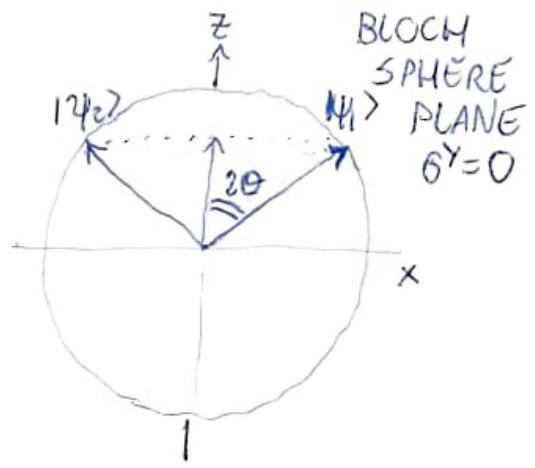
\includegraphics[max width=\textwidth, center]{2025_10_16_1bd50d0393172dac5e59g-02}\\
$50 / 50$ HIXTURE $\quad \begin{cases}\left|\psi_{1}\right\rangle & p=\frac{1}{2} \\ \left|\psi_{2}\right\rangle & p=\frac{1}{2}\end{cases}$

$$
\begin{aligned}
\rho_{0}=\frac{1}{2}\left|\psi_{1} \times \psi_{1}\right|+\frac{1}{2}\left|\psi_{2} \times \psi_{2}\right| & =\frac{1}{2}\left(\begin{array}{cc}
\cos ^{2} \theta & \cos \sin \\
\cos \sin & s^{2}
\end{array}\right)+\frac{1}{2}\left(\begin{array}{cc}
c^{2} & -c s \\
-c s & s^{2}
\end{array}\right) \\
\rho & =\left(\begin{array}{cc}
\cos ^{2} \theta & 0 \\
0 & \sin ^{2} \theta
\end{array}\right) \quad \operatorname{Tr}[\rho]=1 \\
\rho \geqslant 0 &
\end{aligned}
$$

$\rho$ - is $\left.\begin{array}{l}\text { ALSO MIXYRE OF } \\ |0\rangle \text { ANA } H\rangle\end{array}\right\} \quad\left\{\begin{array}{ll}|0\rangle & p=\cos ^{2} \theta \\ |1\rangle & p=\sin ^{2} \theta\end{array} \quad \rho=\cos ^{2} \theta|0 \times 0|+\sin ^{2} \theta|1 \times 1|\right.$

$$
\left\langle\sigma^{z}\right\rangle=\cos 2 \theta \quad\left\langle\sigma^{x}\right\rangle=\left\langle\sigma^{y}\right\rangle=0 \quad \sqrt{ } \text { CHECKS OUT }
$$

$\operatorname{Tr}\left[\rho^{2}\right]=\frac{1}{2}\left(1+\cos ^{2} 2 \theta\right) \xrightarrow{\longrightarrow}\left\{\begin{array}{l}2 \theta=0 \\ 2 \theta=\pi\end{array} \quad\right.$ EXERCISE\\
$|\psi(\varphi)\rangle=\binom{\cos \theta}{e^{i \varphi} \sin \theta}$\\
COMPETE UNCERTAINTY OVER $\varphi$

$$
d p(\varphi)=\frac{1}{2 \pi} d \varphi
$$

$\rho=\int|\psi(\varphi)\rangle\langle\psi(\varphi)| d p(\varphi)=\int_{0}^{2 \pi}\left(\begin{array}{cc}\cos ^{2} \theta & e^{-i \varphi} \sin \theta \cos \theta \\ \text { c.c. } & \sin ^{2} \theta\end{array}\right) \frac{d \varphi}{2 \pi}=\left(\begin{array}{cc}\cos ^{2} \theta & 0 \\ 0 & \sin ^{2} \theta\end{array}\right)$\\
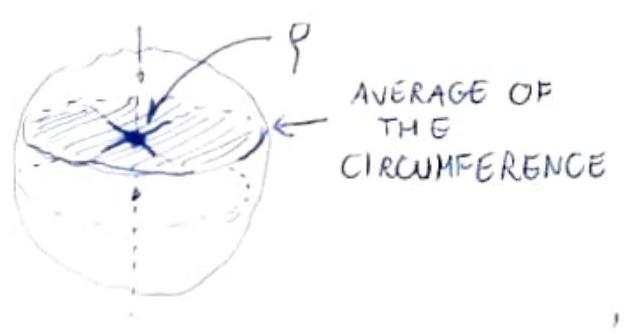
\includegraphics[max width=\textwidth, center]{2025_10_16_1bd50d0393172dac5e59g-03}\\
closed system dynamics for sensity matrices\\
$\rho=\sum_{1} p_{\alpha}\left|\psi_{\alpha} \times \psi_{\alpha}\right|$ NO INTERFERENCE $\Rightarrow$ EVERY MEMBER EVOLVES BY ITSELF PROBABILITIES ARE STATIC $\dot{p}_{2}=0$

$$
\begin{array}{r}
\dot{\rho}=\sum^{\prime} p_{\alpha}\left|\dot{\psi}_{\alpha}\right\rangle\left\langle\psi_{\alpha}\right|+\sum p_{\alpha}\left|\psi_{\alpha}\right\rangle\left\langle\hat{\psi}_{\alpha}\right|=\sum p_{\alpha}\left(-\frac{i}{\hbar} H|\psi \times \psi|+\frac{i}{\hbar}|\psi \times \psi| H\right) \\
=\sum p_{\alpha} \frac{i}{\hbar}\left[i \psi_{\alpha} \times \psi_{\alpha} \mid, H\right]=\left[\sum p_{\alpha}\left|\psi_{\alpha} \times \psi_{\alpha}\right|, H\right] \frac{i}{\hbar}=+\frac{i}{\hbar}[\rho, H] \\
\dot{\rho}=\frac{i}{\hbar}[\rho, H] \quad \begin{array}{l}
\text { SCHOÖSINGER EQ, } \\
\text { FOR SENSITY MATRICES } \\
\text { (SCHR PICTURE) }
\end{array}\left(\begin{array}{c}
\text { SIMICAR TO HEISENBERG } \\
\text { PICURE BUT WITH A } \\
\text { MINUS }
\end{array}\right)
\end{array}
$$

GIBBS/BOLTZMANN\\
ENSEMBLE\\
$\rho=\frac{\exp \left(-\frac{H}{K_{B} T}\right)}{T_{r}\left[\exp \left(-\frac{H}{K_{B} T}\right)\right]}$\\
$\hat{L}$\\
GUANTUH SYSTEH IN CONTACY WITH FIXEST RESERVOIR EQUILIBRATES HERE\\
(1.) STATIONARY $\leftrightarrow$ EQUILIBRIUM\\
(2.) MAXIHISES $S$ AT FIXED INTERNAL ENERGY Tr [Hg] -OR-\\
(3.) HINIMIZES THE FREE ENERGY $F=\operatorname{Tr}[\mathrm{Hp}]-T S(\rho)$ at fixed $T$ TEMPERAYURE

FUT HOW TO GET THERE?

DIPARTTE SYSTEM $A$ B

$$
\left|\psi_{A B}\right\rangle=\sum_{a b} C_{a b}\left|\psi_{a}\right\rangle_{A} \underset{\uparrow}{\otimes}\left|\phi_{b}\right\rangle_{B}
$$

tensur product structure\\
an cbservabe Acting oncy on $A$

$$
\begin{aligned}
C_{A B}=\theta_{A} \otimes \mathbb{1}_{B} \quad\langle\theta\rangle & =\operatorname{Tr}\left[\left(\theta_{A} \otimes \mathbb{1}_{B}\right) \rho_{A B}\right]= \\
& =\sum_{a b}\left\langle\left.\left. a\right|_{A}\left\langle\left.\left. b\right|_{B}\left(\theta_{A} \otimes \frac{1}{B}\right) \rho_{A B} \right\rvert\, a\right\rangle_{A} \right\rvert\, b\right\rangle_{B} \\
& =\sum_{a b}\langle a| \theta_{A}\left\langle\left. b\right|_{B} \rho_{A B} \mid b\right\rangle_{B}|a\rangle_{A}= \\
& =\sum_{a}\langle a| \theta_{A} \rho_{A}|a\rangle=\operatorname{Tr}\left[\theta_{A} \rho_{A}\right]
\end{aligned}
$$

WHERE

$$
\rho_{A}=\Delta \sum_{b}^{1}\left\langle\left. b\right|_{B} \rho_{A B} \mid b\right\rangle_{B}=T_{B}\left[\rho_{A B}\right] \quad \text { TRACE (over B) }
$$

\begin{figure}[h]
\begin{center}
  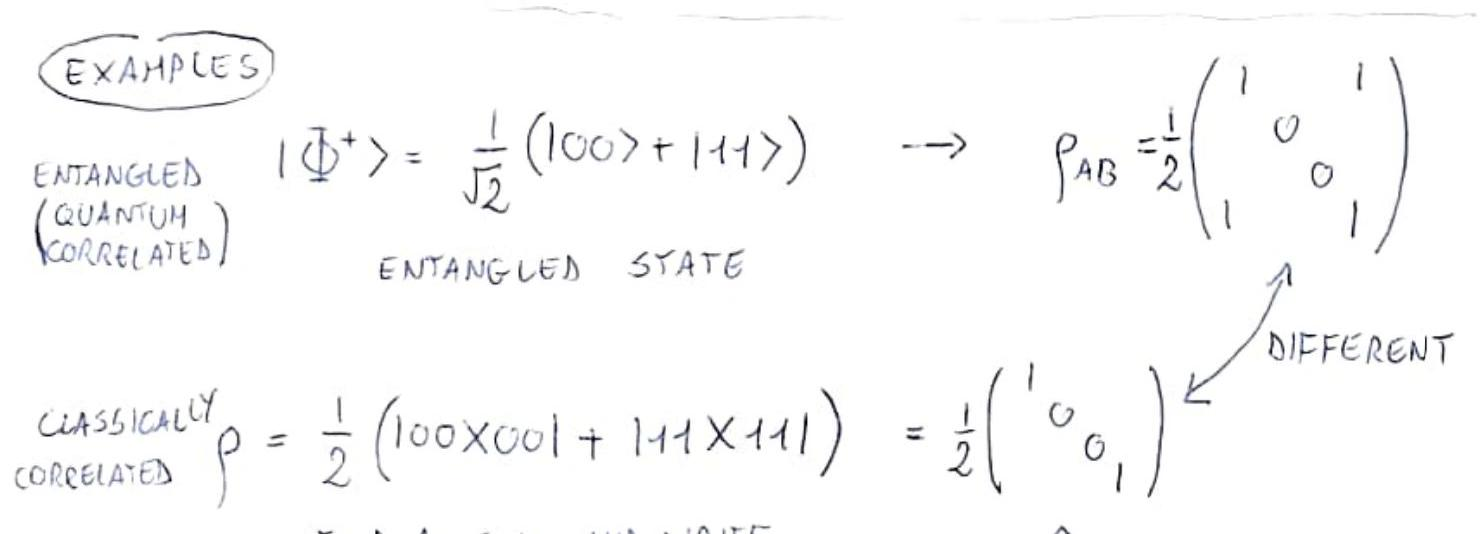
\includegraphics[width=\textwidth]{2025_10_16_1bd50d0393172dac5e59g-04}
\captionsetup{labelformat=empty}
\caption{介\\
NOT ENTANGED}
\end{center}
\end{figure}

$$
\rho_{A}=\frac{1}{2}\left(\begin{array}{ll}
1 & 0 \\
0 & 1
\end{array}\right)=\frac{1}{2}
$$

completecy mixed

$$
\rho_{A}=\frac{11}{2} \text { SAME }
$$

FLIP A COIN AND WRITE the result twice

UNCCRRELAYED

$$
\rho=\frac{11}{2} A \otimes \frac{11}{2} B=\frac{1}{4}\left(\begin{array}{l}
1 \\
1 \\
1
\end{array}\right) \quad \rho_{A}=\frac{11}{2} \underset{\text { SAME }}{\text { CTME }}
$$

THE PARTIAL TRACE\\
HIDES/DELETES/AVERAGES OVER\\
CORRELATIONS (BETWEN A AND B)\\
QUAMTUM OR CLASSICAL

\section*{The Master Equation}
\begin{center}
\begin{tabular}{lll}
SYSTEM $\leftarrow$ & BATH & \begin{tabular}{l}
IN GENERAL, TO DESCRIBE THE SYNAMICS, \\
YOU NEES TO TRACK THE (QUANTUM) EVOLUTION \\
\end{tabular} \\
QUANTUM & \begin{tabular}{l}
QUANTUM \\
AND/OR \\
CLASSICAL \\
\end{tabular} & \begin{tabular}{l}
OF BOTH SYSTEM + BATH TOGETHER \\
TWHEN CAN WE SESCRIBE THE SYSTEM ALONE \\
\end{tabular} \\
 &  & AND DESCRIBE ITS EVOWTION ? \\
\end{tabular}
\end{center}

Born-Markov DYNAMICS\\
! WHEN... THE BATH LOSES IMMEDIATELY MEMORY OF THE SYSTEM (FOR SORE IT WORKS)

\begin{figure}[h]
\begin{center}
  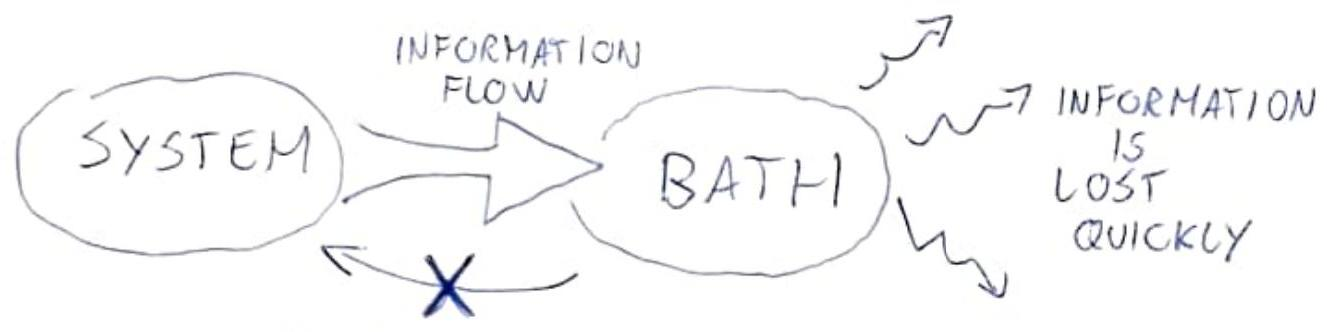
\includegraphics[width=\textwidth]{2025_10_16_1bd50d0393172dac5e59g-05}
\captionsetup{labelformat=empty}
\caption{INFOCMATION NEVER GOES BACK}
\end{center}
\end{figure}

\section*{Physical REQUIREMENT}
the bath must be fast and large\\
(1)

FAST

$$
\begin{aligned}
& H_{\text {TOT }}=H_{\text {SYS }}+H_{\text {BATH }}+H_{\text {WT }} \text { thescale } \\
& \text { SEPARATION } \\
& \tau_{B} \ll \tau_{b} \ll \tau_{\text {INT }} \\
& \text { REQUIRED } \\
& \text { FOR BORN-HARKOV } \\
& \text { APPROX } \\
& \begin{array}{l}
\text { REQUIREA FOR } \\
\text { QUANUM } \\
\text { DYNAMICS }
\end{array} \\
& \text { the bath must have space } \\
& \text { to "STORE AND FORGET" INFO } \\
& \text { about the SYSTEM }
\end{aligned}
$$

$H=H_{S Y S}+H_{\text {BATH }}+H_{\text {INT }} \quad\binom{H_{B}=\mathbb{1}_{S} \otimes H_{B}}{H_{S}=H_{S} \otimes \mathbb{1}_{B}}$\\
Step. 1 change reference frame - interaction pictore\\
$\left[U, H_{3} \otimes \Perp\right]=0<\left[U, 1 \otimes H_{3}\right]$

$$
\begin{aligned}
& \left.\begin{array}{l}
\text { hamiltonian } \\
\text { of the new } \\
\text { frame }
\end{array}\right\}
\end{aligned}
$$

COMPARE WITH THE\\
FORHAL IERIVATION FROM ADSITIVITY

$$
\left(H_{I W T}=\sum_{\alpha}^{1} S_{\alpha} B_{\alpha}\right)
$$

$$
\dot{\rho}^{\prime}(t)=+\frac{i}{\hbar}\left[\rho^{\prime}(t), H_{\text {INT }}(t)\right] \quad \downarrow \text { SIMPLE } \int_{0}^{t} d t
$$

(STEP.2) Integrate and plug-in

$$
\begin{aligned}
& \rho^{\prime}(t)=\rho^{\prime}(0)=\frac{i}{\hbar} \int_{0}^{t}\left[\rho^{\prime}(t), \tilde{H}_{M N}(t)\right] d t \quad\left(\begin{array}{c}
\text { PLUE BACK INSIDE } \\
\text { THE EQUATION } \\
\text { AND GET... } \\
\rho^{\prime}(t)=\rho^{\prime}(0)+\frac{i}{\hbar} \int_{0}^{t}\left[\rho^{\prime}(t), \tilde{H}_{I N T}(t)\right] d t
\end{array}\right. \\
& \dot{\rho}^{\prime}(t)=\underbrace{\frac{i}{\hbar}\left[\rho^{\prime}(0), \tilde{H}_{I N T}(t)\right]}_{\text {PIECE } \Delta}-\underbrace{\frac{1}{\hbar^{2}} \int_{0}^{t}\left[\left[\rho^{\prime}\left(t^{\prime}\right), \tilde{H}_{I N T}\left(t^{\prime}\right)\right], \tilde{H}_{I N T}(t)\right] d t^{\prime}}_{\text {PIECE } \square}
\end{aligned}
$$

BORN APPROXIMATION:

THE STATE OF THE BATH IS UNALTERES\\
$\rho(t)=\rho_{S}(t) \otimes \rho_{B}(0) \underset{\text { FRAME }}{\stackrel{\text { Interation }}{\text { TVAL }}} \rho^{\prime}(t)=\rho_{S}^{\prime}(t) \otimes \rho_{B}(0) \quad\binom{\left.H_{B}+H_{S}\right]}{\rho_{B}^{\prime}=\rho_{B}}$\\
$\operatorname{Tr}_{B}[$ PIECE $\Delta]=\frac{i}{\hbar} \operatorname{Tr}_{B}\left(\left[\rho_{S}^{\prime}(0) \otimes \rho_{B}(0), \check{H}_{\text {INY }}(t)\right]\right)=$\\
$=\frac{i}{\hbar} \sum_{\alpha}\left(\left[\rho_{s}^{\prime}(0), \tilde{S}_{\alpha}(t)\right] \operatorname{Tr}\left(\rho_{\beta}(0) \tilde{B}_{\alpha}(t)\right)\right)=\frac{i}{\hbar} \sum\left\langle\tilde{B}_{\alpha}\right\rangle\left[\rho_{s}^{\prime}(0), \tilde{S}_{\alpha}(t)\right]$\\
REDEFINE THE MODEL\\
$H_{s} \rightarrow H_{s}+\sum S_{\alpha}\left\langle B_{\alpha}\right\rangle$\\
$H_{I N T} \rightarrow \sum_{1} S_{\alpha}\left(B_{\alpha}-\left\langle B_{\alpha}\right\rangle\right)$\\
The second piece\\
The second piece\\
$\dot{\rho}_{S}^{\prime}(t)=+\frac{1}{\hbar^{2}} \int_{0}^{t} T_{B}\left(\left[\left[\tilde{H}_{\text {INT }}\left(t^{\prime}\right), \rho_{S}^{\prime}\left(t^{\prime}\right) \otimes \rho_{B}(0)\right], \tilde{H}_{\text {INT }}(t)\right]\right) d t^{\prime}$ NAKAJIMA-ZOWANZIG EQUATION

AFTER THIS RE-SEFINITION THE NEW $\left\langle B_{\alpha}\right\rangle=0$

$$
T_{B}(P \mid E C E \Delta)=0 .
$$

$$
H_{I N T}=\sum_{\alpha} S_{\alpha}^{e} B_{\alpha}=\sum S_{\beta}^{+} \otimes B_{\beta}^{+}
$$

$\dot{\rho}_{S}^{\prime}(t)=\frac{1}{\hbar^{2}} \int_{0}^{t} \tilde{S}_{\alpha}\left(t^{\prime}\right) \rho_{s}^{\prime}\left(t^{\prime}\right) \tilde{S}_{\beta}^{\dagger}(t) \underbrace{\operatorname{Tr}\left[\rho_{\beta}(0) \tilde{B}_{\alpha}\left(t^{\prime}\right) \tilde{B}_{\beta}^{+}(t)\right]}_{\operatorname{Tr}\left[\rho(0) \tilde{B}^{\prime}(0) \tilde{B}^{+}(t-\theta)\right]}+\left(\begin{array}{c}\text { THER } \\ \text { THEREENIS } \\ \text { COMPONENT }\end{array}\right)$

PUTTING PIECES BACK\\
$\dot{\rho}_{S}^{\prime}(t)=+\frac{1}{\hbar^{2}} \sum_{\alpha \beta} \int_{0}^{t}\left\{\mathcal{G}_{\alpha \beta}\left(t-t^{\prime}\right)\left(\tilde{S}_{\alpha}\left(t^{\prime}\right)\right.\right. \left.+C_{\beta \alpha}\left(t^{\prime}-t\right)\left(\breve{S}_{\beta}^{+}(t) \rho_{5}^{\prime}\left(t^{\prime}\right) \breve{S}_{\alpha}\left(t^{\prime}\right)-\rho_{5}^{\prime}\left(t^{\prime}\right) \widehat{S}_{\alpha}\left(t^{\prime}\right) \tilde{S}_{\beta}^{+}(t)\right)\right\} d t$\\
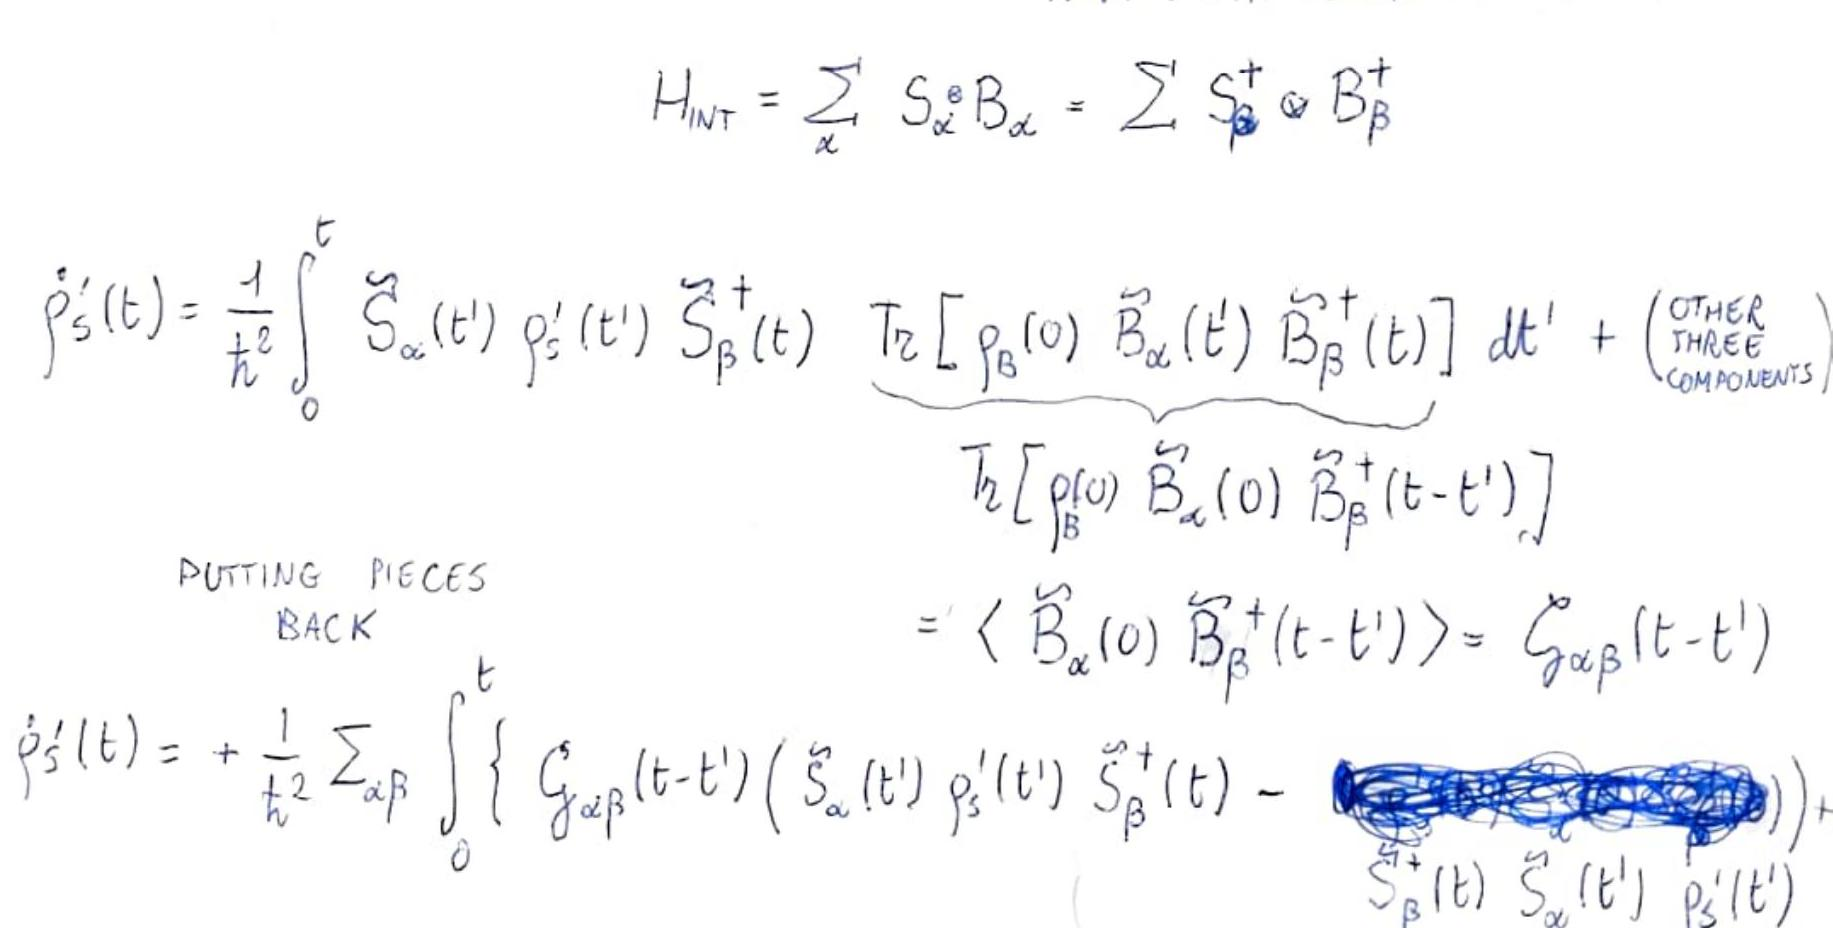
\includegraphics[max width=\textwidth]{2025_10_16_1bd50d0393172dac5e59g-07} ${ }_{\beta}^{+}(t) \tilde{S}_{\alpha}\left(t^{\prime}\right) \rho_{\beta}^{\prime}\left(t^{\prime}\right)$

\section*{MARKOV APPROXIMATION}
the correcations of the bath secay super fast

$$
\begin{array}{r}
\oint_{\alpha \beta}(t) \propto \zeta_{\alpha \beta}(0) \delta(t) \quad \text { 《 FOR SANITY, LET US } \\
\dot{\rho}_{S}^{\prime}(t)=\sum_{\alpha \beta} \zeta_{\alpha \beta}\left(\tilde{S}_{\alpha} \rho_{S}^{\prime} \tilde{S}_{\beta}^{+}-\tilde{S}_{\beta}^{+} \tilde{S}_{\alpha} \rho_{S}^{\prime}\right)_{t}+\zeta_{\beta \alpha}\left(\tilde{S}_{\beta}^{+} \rho_{S}^{\prime} \tilde{S}_{\alpha}-\rho_{S}^{\prime} \tilde{S}_{\alpha} \tilde{S}_{\beta}^{+}\right)
\end{array}
$$

BACK TO THE LAB FRAME $\rho_{5}(t)=e^{-i t H_{5}} \rho_{5} e^{+i t H_{5}}$

$$
\begin{aligned}
& \begin{array}{c}
\dot{\rho}_{S}(t)=+i\left[\rho_{S}^{(t)}, H_{S}\right]+\sum_{\alpha \beta} G_{\alpha \beta}\left(S_{\alpha} \rho_{3}(t) S_{\beta}^{+}-S_{\beta}^{+} S_{\alpha} \rho_{s}(t)\right)+\underbrace{}_{\sum_{\alpha \beta}}\left(S_{\beta}^{+} \rho_{\beta}(t) S_{\alpha}-\rho_{S}(t) S_{2} S_{\beta}^{+},\right. \\
\left\langle B_{\alpha} B_{\beta}^{r}\right\rangle
\end{array} \\
& \text { USING } \begin{array}{ll}
\text { II } & \text { EXTENS } \\
& \sum_{p}^{+} S_{p}^{+} B_{\beta}^{+}
\end{array} \text {VECTOR OF } \\
& C_{\alpha \beta}\left(S_{\alpha} \rho S_{\beta}^{+}-\rho S_{\beta}^{+} S_{\alpha}\right)
\end{aligned}
$$

$$
\rho_{s}=\frac{i}{\hbar}\left[\rho_{s}, H_{s}\right]+\sum_{\alpha \beta} C_{\alpha \beta}\left(2 S_{\alpha} \rho S_{\beta}^{+}-\left\{S_{\beta}^{+} S_{\alpha}, \rho\right\}\right)
$$

$$
\begin{aligned}
& G_{\alpha \beta}=\operatorname{Tr}\left[\rho_{\beta} B_{\alpha} B_{\beta}^{+}\right] \rightarrow G_{\alpha \beta} \quad \begin{array}{c}
\text { IS POSITIVE } \\
\text { SEMISEINITE }
\end{array} \rightarrow \begin{array}{c}
\text { CAN BE } \\
\text { DIAGONALIZES } \\
u_{\alpha Y}^{+} \gamma_{j}^{N} u_{j \beta} \\
\text { REDEFINE } L_{j}=\sum_{\alpha} u_{j, \alpha} S_{\alpha} \sqrt{2}
\end{array}
\end{aligned}
$$

DIMENSIONLESS LINDBLADIANS

$$
\begin{array}{r}
\dot{\rho}_{S}=\frac{i}{\hbar}\left[\rho_{1} H_{3}\right]+\sum_{J} \int_{\prod_{S}}\left(L_{J}^{\downarrow} \rho L_{J}^{+}-\frac{1}{2}\left\{L_{J}^{+} L_{J}, \rho\right\}\right) \\
\geqslant 0 \text { DIMENSION OF } t^{-1} \quad \rho=\mathcal{L}(\rho)
\end{array}
$$

lindscas master equation

NOTICE $\frac{d}{d t} T r[\rho]=0 \leftarrow$ no coss of tOTAL PROBABICITY\\[0pt]
example 1 [harkovian dynamics] Decay

2-hevel system

\begin{itemize}
  \item ${ }^{|e\rangle}$
\end{itemize}

$$
H_{s}=\hbar \omega|e \times e|
$$

$\frac{\sum_{2}}{|y|}$\\
ONE

$$
\rho_{0}=\left(\begin{array}{ll}
a_{0} & b_{0} \\
b_{0}^{*} & c_{0}
\end{array}\right)
$$

WHERE

$$
c_{0}=1-a_{0}
$$

$\underbrace{\left|b_{0}\right|^{2} \leqslant a_{0} c_{0}}_{\substack{\text { POSITIVITY } \\ \text { CONDITION }}}$

$$
\rho(t)=\left(\begin{array}{ll}
a(t) & b(t) \\
b^{*}(t) & c(t)
\end{array}\right)
$$

$\dot{\rho}(t)=-\frac{i}{\hbar} H_{\downarrow} \rho+\frac{i}{\hbar} \rho H+\gamma L \rho L^{+}-\frac{1}{2} \gamma L^{+} L \rho-\frac{\gamma}{2} \rho \underbrace{\rho L^{+} L}_{\downarrow}$\\
$H=\hbar \omega\left(\begin{array}{ll}0 & 0 \\ 0 & 1\end{array}\right) \quad\left(\begin{array}{ll}0 & 1 \\ 0 & 0\end{array}\right) \quad\left(\begin{array}{ll}0 & 0 \\ 1 & 0\end{array}\right) \quad\left(\begin{array}{ll}0 & 0 \\ 0 & 1\end{array}\right)$\\
$\left(\begin{array}{cc}\dot{a} & \dot{b} \\ \dot{b} & \dot{c}\end{array}\right)=i \omega\left(\left(\begin{array}{ll}0 & b \\ 0 & c\end{array}\right)-\left(\begin{array}{cc}0 & 0 \\ b^{*} & c\end{array}\right)\right)+\gamma\left(\left(\begin{array}{ll}c & 0 \\ 0 & 0\end{array}\right)-\frac{1}{2}\left(\begin{array}{ll}0 & 0 \\ b^{*} & c\end{array}\right)-\frac{1}{2}\left(\begin{array}{ll}0 & b \\ 0 & c\end{array}\right)\right)$\\
DIFFERENTIAC EQCATIONS FOR $b$ ANS $c \rightarrow$ EASY

$$
\begin{cases}\begin{array}{l}
\dot{b}=\left(i \omega-\frac{\gamma}{2}\right) b(t) \\
\dot{c}=-\gamma c(t)
\end{array} \Rightarrow & b(t)=b_{0} e^{\left(i \omega-\frac{\gamma}{2}\right) t} \ll \text { SPIRAL } \\
a=(1-c) & c(t)=c_{0} e^{-\gamma t} \geqslant 0 \\
\rho(t)=\left(\begin{array}{cc}
1-c_{0} e^{-\gamma t} & e^{\left(i \omega-\frac{\gamma}{2}\right) t} b_{0} \\
e^{\left(-i \omega-\frac{\gamma}{2}\right) t} b_{0}^{*} & c_{0} e^{-\gamma t}
\end{array}\right) \\
\downarrow t \rightarrow \infty \text { STEADY STATE } \\
\rho(t=\infty)=\left(\begin{array}{ll}
1 & 0 \\
0 & 0
\end{array}\right)=|g \times g|\end{cases}
$$

\section*{Example 2 Dephasing}
$$
L=L^{+}=L^{+} L=\left(\begin{array}{ll}
0 & 0 \\
0 & 1
\end{array}\right)=H \frac{1}{\hbar \omega}
$$

$$
\begin{aligned}
& H=\hbar \omega(e \times e) \\
& L=|e \times e| \text { ANE } \gamma\left\{\begin{array}{l}
\text { PROBABILIST } \\
\text { FUPP }
\end{array}\right.
\end{aligned}
$$

$\left(\begin{array}{cc}\dot{a} & \dot{b} \\ b^{*} & \dot{c}\end{array}\right)=i \omega\left(\begin{array}{cc}0 & b \\ b^{*} & 0\end{array}\right)+\gamma\left(\left(\begin{array}{ll}0 & 0 \\ 0 & c\end{array}\right)-\frac{1}{2}\left(\begin{array}{ll}0 & b \\ 0 & c\end{array}\right)-\frac{1}{2}\left(\begin{array}{ll}0 & 0 \\ b^{*} & c\end{array}\right)\right) c(t)=c_{0} \quad a(t)=1-c_{0} \quad b(t)=e^{\left(i \omega-\frac{r}{2}\right) t} b_{0}$

$$
\begin{aligned}
& \left\langle\sigma^{2}\right\rangle(t)=a(t)-c(t)=1-2 c_{0} \text { constant } \\
& \left\langle\sigma^{*}\right\rangle(t)=\operatorname{tr}\left[\left(1^{\prime}\right)\left(\begin{array}{ll}
a & b \\
b^{*} c
\end{array}\right)\right]=b+b^{*}=e^{-\frac{\gamma}{2} t} \operatorname{Re}\left(e^{i \omega t} b_{0}\right)
\end{aligned}
$$

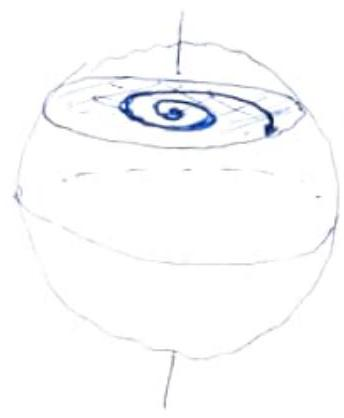
\includegraphics[max width=\textwidth, center]{2025_10_16_1bd50d0393172dac5e59g-10}\\
$\leftarrow$ Trasectory:

$$
\left(b_{0} R E A L\right)=e^{-\frac{\gamma}{2} t} \cos (\omega t) b_{0}
$$

IN-PLANE SPIRAL\\
steady syate(s)

$$
\rho(t=\infty)=\left(\begin{array}{cc}
1-c_{0} & 0 \\
0 & c_{0}
\end{array}\right)
$$

NON-ONIQUE because of CONSERVES $\left\langle\sigma^{z}\right\rangle$

Dephasing 2.0\\
$p_{\substack{F_{1} x \in D \\ \omega}}(t)=\left(\begin{array}{cc}1-c_{0} & b_{c} e^{+i \omega t} \\ b_{0}^{*} e^{-i \omega t} & c_{0}\end{array}\right)$\\
$\int_{\substack{\text { HEMSTICONNN } \\ \text { ENSEHRE }}}$

$$
\begin{array}{r}
=\left(\begin{array}{cc}
1-c_{0} & b_{0} \int e^{i \omega t}\left(\frac{d \rho}{d \omega}\right) d \omega \\
c & c_{0}
\end{array}\right) \\
\rho_{t>0}(t)=\left(\begin{array}{cc}
1-c_{0} & e^{\left(i \omega_{0}-\gamma\right) t} \\
c . c & c_{0}
\end{array}\right)
\end{array}
$$

no bath but cuasical

$$
H=\text { iexei } \hbar \omega
$$

probability density $\overbrace{\text { RANDOM }}^{\text {VARIABLE (STATIC) }}$

$$
\left\{\begin{array}{l}
\int \frac{d p}{d \omega} \cdot d \omega=\int d p(\omega) \\
\frac{d p}{d \omega}=\frac{1}{\pi} \frac{\gamma}{\left(\omega-\omega_{0}\right)^{2}+\gamma^{2}} \\
\text { (AUCHY-CORGNZIZ SISTRP) }
\end{array}\right.
$$

BUT $\int_{-\infty}^{+\infty} \frac{d \omega}{\pi} \frac{\gamma e^{i \omega t}}{\left(\omega-\omega_{0}\right)^{2}+\gamma^{2}}=e^{i \omega_{0} t-\gamma|t|} \leftarrow \quad$ IDENTICAL TO PREVIOUS\\
EXERCISE. HARKOUAT DYNAMICS\\
ALSO MODELS NOISE (SOME FORHS)\\
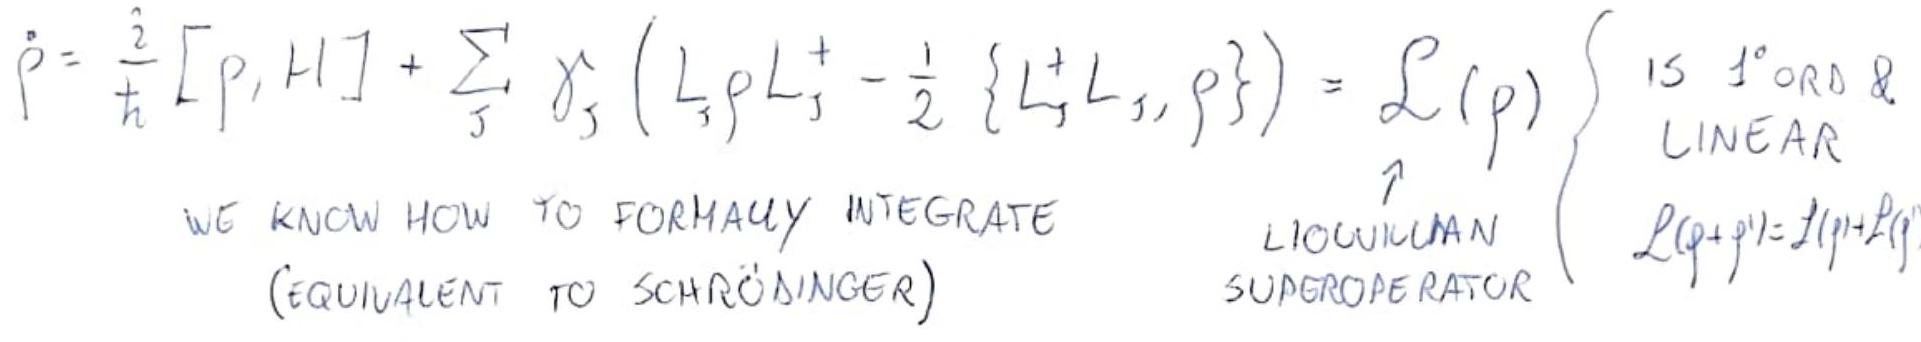
\includegraphics[max width=\textwidth, center]{2025_10_16_1bd50d0393172dac5e59g-11}\\
TURN $\rho$ FROM matrix to vector $\hat{\rho} \rightarrow|\rho\rangle\rangle \quad \hat{\rho}$ SIMENSION $d_{H} \times d_{H}$\\
UKE THIS $|i\rangle\langle J| \rightarrow|i J\rangle\rangle$

$$
|p\rangle \text { SIMENSION } d_{H}^{2} \times 1
$$

$$
\stackrel{\text { SO THAT }}{\longrightarrow}\left(\begin{array}{ll}
a & b \\
c & d
\end{array}\right) \rightarrow\left(\begin{array}{l}
a \\
b \\
c \\
d
\end{array}\right) \quad \begin{gathered}
\text { SOMESTHES } \\
\text { KNOWN AS } \\
\text { CHOI TRANSFORY }
\end{gathered}
$$

PROPERTIES\\
HILBERT-SCHMIAT PRODUCY ON OPS\\
$T_{r}\left[o_{p}\right]=$\\
$A p B \xrightarrow{C 401} A \otimes B_{\text {TRAN SDOSE }}^{t}|p\rangle$

$$
\begin{aligned}
\operatorname{Tr}\left[A^{+}, B\right] & =(A, B) \\
& =\langle\langle A \mid B\rangle\rangle
\end{aligned}
$$

IN CANONCAL BASIS

$$
\left.\left.=\langle\| 1| \sigma_{\theta} 1|\rho\rangle\right\rangle=\langle\langle 1| 1| \otimes \sigma^{*}|\rho\rangle\right\rangle=\left\langle\left\langle\theta^{(t)} \mid \rho\right\rangle\right\rangle
$$

hataix ecemeny

$$
\rho_{i j}=\langle i| \rho|j\rangle=\langle\langle i j \mid \rho\rangle\rangle
$$

The llouviulan as supermatrix $\hat{\hat{L}}$ (in choi teansform)\\
$\left.|\dot{\rho}\rangle\rangle=\hat{\mathcal{L}}_{\hat{\rho}}^{\hat{\alpha}}|\rho\rangle\right\rangle=\left(-\frac{i}{\hbar} H \otimes \mathbb{1}+\frac{i}{\hbar} \mathbb{1} \otimes H^{*}+\sum_{J} \chi_{J}\left(L_{J} \otimes L_{J}^{*}\right.\right.$

IF $\mathcal{L}$ に\\
time independent

$$
\left.\left.\left.\left.-\frac{1}{2} L_{J}^{+} L_{J} \otimes \mathbb{1}-\frac{1}{2} \mathbb{1} \otimes L_{J}^{t} L_{J}^{*}\right)\right) d \rho\right\rangle\right\rangle
$$

HOWEVER $\hat{l}$ IS NOT HERMITIAN.\\
$|\rho(t)\rangle\rangle=\exp ($ 总 $\left.t)\left|\rho_{0}\right\rangle\right\rangle$\\
IFE $\mathcal{L}$ CAN BE SIAGONACIZES $\quad \times D X^{-1}$

$$
\left.|\rho(t)\rangle\rangle=x e^{D t} x^{-1}\left|\rho_{0}\right\rangle\right\rangle
$$

(A) Exploding solutions are not physical, so $\forall \lambda \in D, \operatorname{Re}(\lambda) \leqslant 0$ negative real part\\
(B) Steady state $|\dot{p}\rangle\rangle=0 《 \Leftrightarrow\rangle \quad \hat{\hat{\mathcal{L}}}|\rho\rangle\rangle=0$ FOR THE LIOUVILIAN SPEC\\
ipst most be in the KERNEL of $\mathcal{L}$\\
! NOT ALL EIGENVECTORS ARE DENSITY MATRICES!\\
IN FACT

$$
\left.\left(\begin{array}{l}
1 \\
0 \\
0 \\
1
\end{array}\right)=|\mathbb{1}|>\right\rangle
$$

$|\dot{\rho}\rangle\rangle=\mathcal{L}|\rho\rangle\rangle$ meserves the norm $\operatorname{Tr}[\rho]=\operatorname{Tr}\left[j^{+} \rho\right]=\langle\langle\mathbb{I} \mid \rho\rangle\rangle$\\
$\left.\left.\left.{ }_{\text {IHIS }}^{\text {THES }} \rightarrow \underline{\mathcal{L}|v\rangle}=\lambda|v\rangle\right\rangle \quad|v(t)\rangle\right\rangle=e^{\lambda t}\left|v_{0}\right\rangle\right\rangle$ if $\operatorname{Re}(\lambda)<0$ EIGENVECTOR

$$
\operatorname{Tr}\left[v_{0}\right]=\operatorname{Tr}[v(t)]=\sum_{<1}^{e^{\lambda t}} \operatorname{Tr}\left[v_{0}\right]
$$

$\left\{\begin{array}{l}\text { ALL DECAYING } \\ \text { EIGEN-SUPERVECTORS } \\ \text { ARE TRACELESS }\end{array}\right.$\\
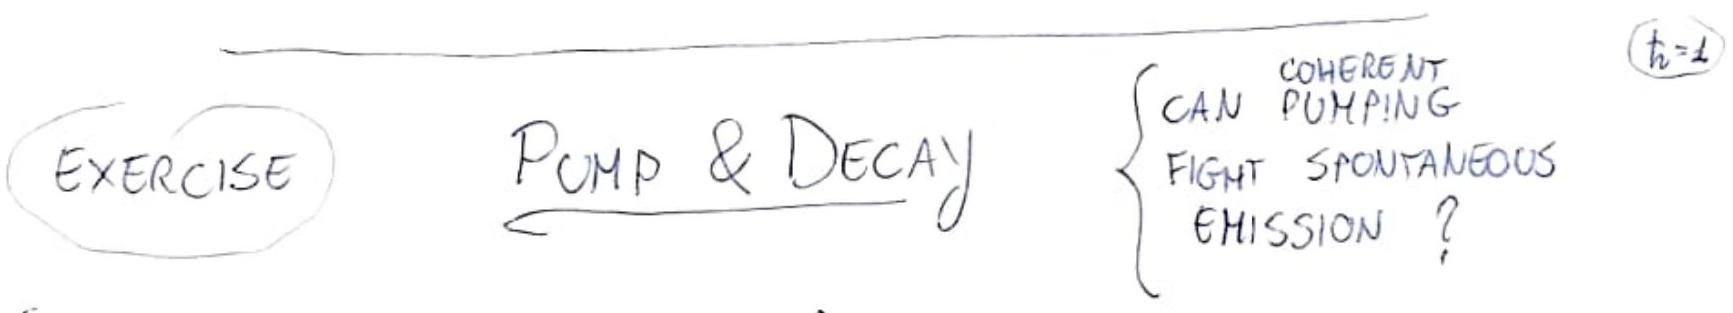
\includegraphics[max width=\textwidth, center]{2025_10_16_1bd50d0393172dac5e59g-12(1)}\\
$\left\{\begin{array}{l}H=\Omega \sigma^{x}=\Omega(|g\rangle\langle e|+|e\rangle \\ L=|g\rangle\langle e| \text { WIH RATE } \gamma\end{array}\right.$

$$
e\rangle\langle g|)
$$

$\sigma^{+}$

$$
H=\Omega\binom{1}{1} \quad L=\left(\begin{array}{ll}
0 & 1 \\
0 & 0
\end{array}\right) \quad L^{+} L=\left(\begin{array}{ll}
0 & 0 \\
0 & 1
\end{array}\right)
$$

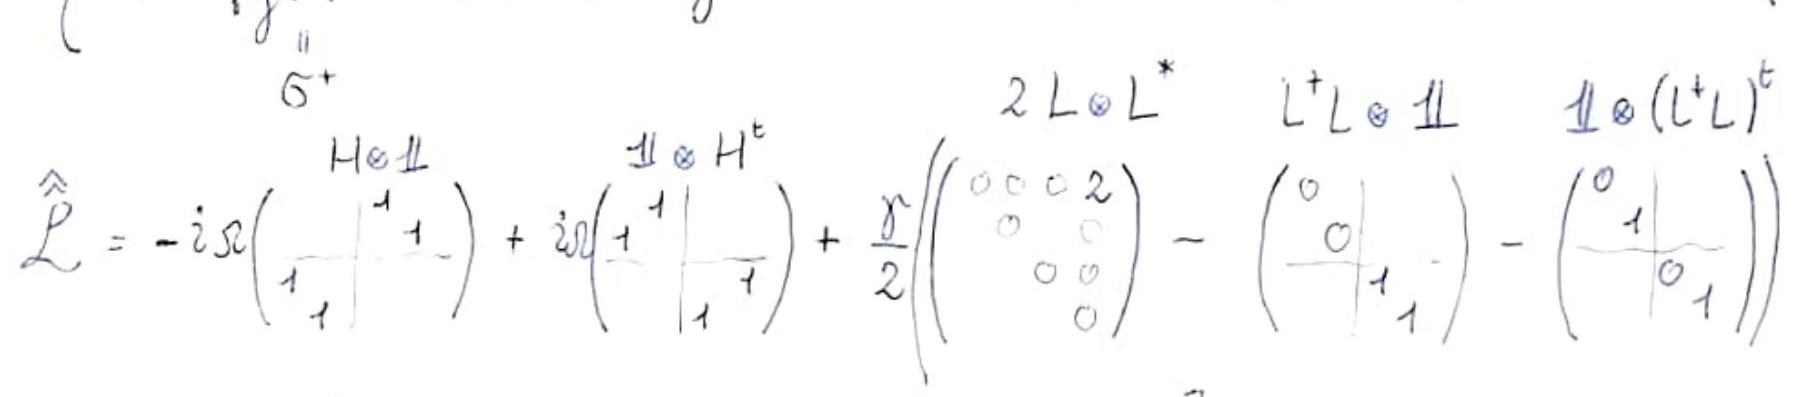
\includegraphics[max width=\textwidth, center]{2025_10_16_1bd50d0393172dac5e59g-12}\\
$\hat{\mathcal{L}}=\Omega\left[\left(\begin{array}{cccc}0 & i & -i & \\ i & 0 & & -i \\ -i & & 0 & i \\ & & -i & i \\ & & 0\end{array}\right)+\frac{\gamma}{2 \Omega}\left(\begin{array}{lll}0 & & \\ & -1 & \\ & & -1 \\ & & \\ & & \\ & & \end{array}\right)\right]$


\end{document}